\documentclass[a4paper,12pt,french]{article}
%Déclaration des packages

\usepackage[latin1,utf8]{inputenc}  
\usepackage{ucs}
\usepackage{url}
\usepackage[babel=true]{csquotes}
\usepackage{amsfonts,amsmath,amsthm}
\usepackage[french]{babel}
\usepackage{graphicx}
\usepackage{tikz}
\usepackage{lscape}
\usepackage{chngpage}
\usepackage{pifont}
\usepackage{listingsutf8}
\usepackage{listings}
\usepackage{color}
\usepackage[T1]{fontenc}
\usepackage{hyperref}
\usepackage{enumitem}
\newcommand{\ul}{\underline}

\lstset{inputencoding=utf8/latin1}
\lstnewenvironment{code}[1][]{  
 \lstset{
  basicstyle=\largel,
  columns=flexible,
  basicstyle=\ttfamily,
  language=Python,  % On choisit le language qui sera utilise dans cet environnement
  morekeywords={input},
  keywordstyle=\color{blue},  % On choisit la couleur des mots cles (def, while, if, for, try et tous les autres) de python
  commentstyle=\color{red!90},  % On choisit la couleur des commentaires
  breaklines,
  breakindent=1em, % On regle l'espacement pour l'indentation
  xleftmargin=0.2em, % On regle la marge de gauche (a l'interieur de la "boite" de code)
  xrightmargin=0.2em, % On choisit la marge de droite
  frame=single,
  rulecolor=\color{orange},
  backgroundcolor=\color{yellow!40}, % Le fond est a 30% de couleur jaune
  #1
 }
}{}

\setlength\fboxrule{1pt}


% Début du document
\begin{document}
\title{Rapport Projet de Synthèse}
\author{Marius AMBAYRAC et Andrés Garcia}
\date{2018}
\maketitle
\clearpage
\tableofcontents
\clearpage

\section{Introduction}
% Idée : On explique ce qu'est le codage,
% Introduire à la fois le codage canal et le codage de source puis
% expliquer que l'on va s'intéresser en priorité au codage de source

\section{Partie Théorique}
% Développer les différents aspects du codage de source

	\subsection{Définitions essentielles}
	% On introduit ici les définitions de base, les autres seront introduites au fur et à mesure, plus tard
	
	\subsection{Inégalité de Kraft-McMillan}
	
	\subsection{Bornes sur la longueur moyenne attendue d'un code}
	
	\subsection{Optimalité du Codage de Huffmann}
	
	\subsection{Limitations du Codage de Huffmann}
	
\section{Partie pratique}

	\subsection{Source binaire sans mémoire}
	
	\subsection{Source binaire Markovienne}
	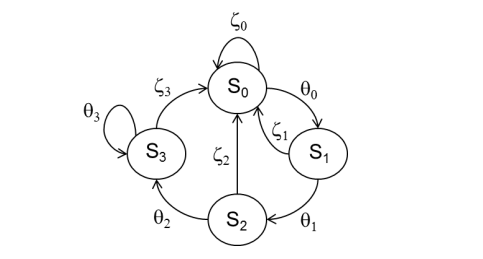
\includegraphics[scale=1]{SourceAvecMemoire.png}
	
\section{Bibliographie}
 	
\section{Annexe}	
	\subsection{Petites Fonctions}
		\subsubsection{Calcul de l'entropie}
		\begin{code}
		def entropie(tab_proba):
    '''Cette fonction calcule l'entropie du tableau de probabilité fourni en entrée sous la forme de tuple (frequence, motif)'''
    somme = 0
    for (pi,elm) in tab_proba:
        somme += pi*log(pi,2)
    return -somme
		\end{code}
		\subsubsection{Longueur moyenne d'un codage}
		\begin{code}
		def longueur_moyenne(source,codage):
    '''Cette fonction calcule la longueur moyenne d'un codage. Elle prend en entrée une liste de tuple (frequence,motif) et une autre liste de tuple (code, motif).'''
    long = 0
    for (freq,motif) in source:
        for (code,motifBis) in codage :
            if motif==motifBis :
                long += len(code)*freq
    return long
    \end{code}
	\subsection{Codage de Hamming}
	\begin{code}
	def Huffman(tab_proba):
    """Cette fonction prend en entrée une liste de tuple (frequence,motif)
    et retourne une liste de tuple (code, motif)"""
    m = len(tab_proba)
    C = [("0","Initial")]*m                                                                #C est le tableau de tuple que l'on renverra, il est composé de (code, motifACoder)
    if m == 2 :                                                                            #Cas de base de notre algorithme récursif
        C[0],C[1] = ("0",tab_proba[0][1]),("1",tab_proba[1][1])
    else :
        tab_proba.sort(reverse = True)                                                     #On trie la liste des proba dans le sens décroissant
        temp = Huffman(tab_proba[0:-2] + [(tab_proba[-2][0]+tab_proba[-1][0],"new")])      #On applique le procédé sur une liste de taille m-1
        indice = recup(temp,"new")                                                         
        #On regarde ou l'élément "spécial" s'est positionné suite au tri
        temp.append(temp[indice])
        temp.pop(indice)                                                                    #On l'enlève pour le repositionner à la fin de la liste
        for i in range(m-2):                                                                #On récupère les codes pour les m-2 premiers motifs
            C[i] = temp[i]
        C[m-2] = (temp[-1][0]+"0",tab_proba[-2][1])                                         #On crée les codes pour les 2 derniers motifs
        C[m-1] = (temp[-1][0] + "1",tab_proba[-1][1])
    return C
	\end{code}
\end{document}